\documentclass[a4paper,12pt]{article}
\usepackage[margin=1in]{geometry}

\usepackage[T2A]{fontenc}			% кодировка
\usepackage[utf8]{inputenc}			% кодировка исходного текста
\usepackage[english,russian]{babel}	% локализация и переносы
\usepackage{graphicx}                % Математика
\usepackage{amsmath,amsfonts,amssymb,amsthm,mathtools} 
\usepackage{mathtext}
\usepackage[T2A]{fontenc}
\usepackage[utf8]{inputenc}

\usepackage{wasysym}

%Заговолок
\author{Бичина Марина 
группа Б04-005 1 курса ФЭФМ}
\title{}
\date{}


\begin{document} % начало документа

\begin{center}
\begin{Large}
{Корнеев Николай Б04-005, Лабораторная работа №. 4.4.1, Изучение амплитудной дифракционной решетки}
\end{Large}
\end{center}
\paragraph{Цель работы: } 
\begin{enumerate}
\itemsep0em
\item Ознакомиться с устройством, работой и настройкой гониометра Г5
\item Отъюстировать гониометр
\item Исследовать спектр ртутной лампы
\item Определить период и спектральные характеристики решетки
\end{enumerate}
\paragraph{Оборудование:}
\begin{enumerate}
\itemsep0em
\item гониометр
\item дифракционная решетка
\item ртутная лампа
\end{enumerate}


\paragraph{Теоретическая справка:} Оптические приборы, в которых осуществляется физическое разложение электромагнитного излучения на монохроматические составляющие, называются спектральными. По характеру распределения интенсивности в спектральном разложении спектры могут быть разделены на линейчатые, непрерывные или сплошные. В нашем лабораторном практикуме исследуются линейчатые спектры. \\
Можно рассмотреть 3 наиболее важные характеристики, на которые мы обращаем внимание, говоря о данном типе оптических приборов:
\begin{enumerate}
\itemsep0em
\item Разрешающая способность $R = \dfrac{\lambda}{\delta \lambda}$ - возможность различать 2 близкие спектральные линии
\item Угловая дисперсия $D = \dfrac{d\phi}{d\lambda}$ - производная зависимости угла отклонения волны диспергирующим элементом по длине волны. По данной величине можно определить угловое расстояние между двумя близкими спектральными линиями $\delta\phi = D\delta\lambda$
\item Дисперсионная область - предельная ширина спектрального интервала прибора, для которой дифракционные максимумы соседних порядков не перекрываются.
\end{enumerate}
Также, говоря о дифракционной решетке, есть основное соотношение приближенной теории дифракционной решетки: 
$d\sin\phi_m = m\lambda$, откуда можно получить выражение для угловой дисперсии:
 $D = \dfrac{d\phi}{d\lambda} = \text{(для дифракционной решетки)} =\dfrac{m}{d \cdot cos\phi} = \dfrac{m}{\sqrt{d^2-(m\lambda)^2}}$ (1)\\
 Разрешающую способность, в силу критерия Релея, можно записать как: $R = Nm$ (2)

\paragraph{Описание установки:}

Говоря об устройстве гониометра, опишем лишь некоторые обозначенные на рисунке гониометра элементы:\\ 
23 -- массивное основание. На нем крепятся:\\
3 - коллиматор\\
7 - столик, на котором размещаются исследуемые объекты(дифракционная решетка, призма)\\
17 - алиада\\
12 - зрительная труда \\
Коллиматор закреплен неподвижно, а столик, алиада, труба - могут вращаться вокруг вертикальной оси
\begin{figure}[h!]
\centering
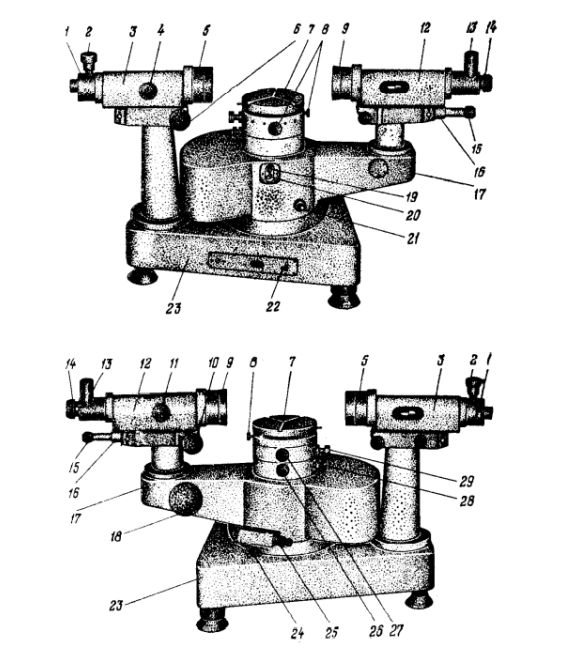
\includegraphics[scale=0.7]{goniometr.png}
\caption{Гониометр} 
\end{figure}\\
\textbf{Спектр ртутной лампы:}
Ниже приведены некоторые интегральные характеристики спектральных линий для лампы ДРШ-250:
\begin{figure}[h!]
\centering
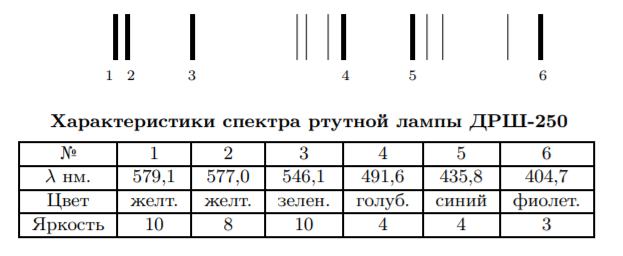
\includegraphics[scale=1]{spectr.png} 
\end{figure}
\paragraph{Ход работы:}
\begin{enumerate}
\itemsep0em
\item Зададим начало отсчета: $180^o11"00'$. Далее значения указываются за вычетом нулевой координаты
\item Измерим угловые координаты спектральных линий ртути. Вычислим синусы от угловых координат. Результаты занесем в таблицу\\
\\
\begin{tabular}{|c|c|c|c|c|c|c|}
\hline 
Цвет & Синий & Голубой & Зеленый & Желтый & Желтый & Красный \\ 
\hline 
$\phi$ & $12^054'46"$ & $14^042'10"$ & $15^058'36"$ & $16^053'41"$ & $16^057'27"$ & $17^057'27"$ \\ 
\hline 
$\sin\phi$ & 0.2234 & 0.2538 & 0.2752 & 0.2906 & 0.2917 & 0.3083 \\ 
\hline 
$\lambda$, нм & 435.8 & 491.6 & 546.1 & 577 & 579.1 & 623.4 \\ 
\hline 
\end{tabular}\\ 
\item Построим график зависимости длины волны от синуса угловой координаты, взяв за погрешность измерения угловой координаты 1 секунду:
$$sin(1") = 8.7\cdot10^{-8}$$
График будем строить основываясь на методе наименьших квадратов:
\begin{equation*}
b = \frac{\langle xy \rangle - \langle x \rangle \langle y \rangle}{\langle x^2 \rangle - \langle x \rangle^2} \;\;
a = \langle y \rangle - b \cdot \langle x \rangle
\label{mnk}
\end{equation*}
\begin{figure}[h!]
\centering
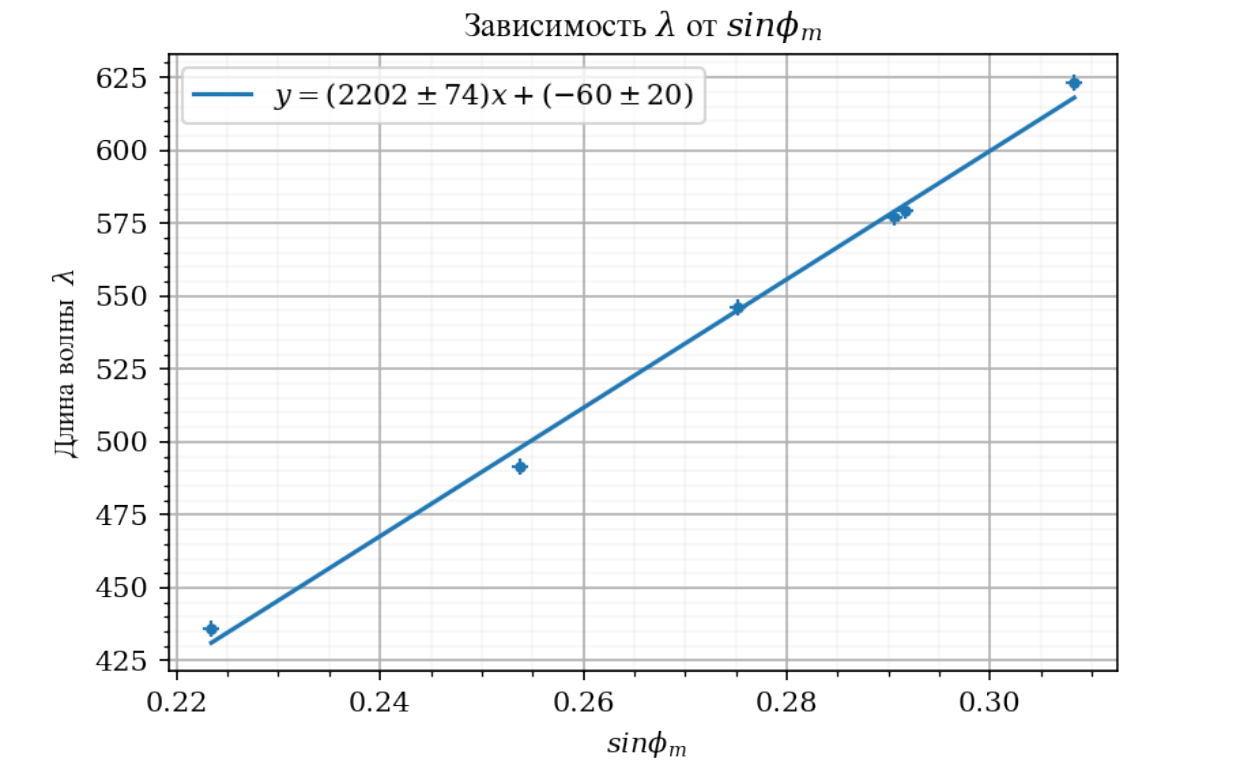
\includegraphics[scale=0.4]{plot.png} 
\end{figure}
\item Рассчитаем угловую дисперсию, зная, что период решетки равен угловому коэффициенту графика d = 2200 нм = 2.200 $\pm$ 0.074 мкм по формуле (1)
\begin{center}
\begin{tabular}{|c|c|c|c|c|c|}
\hline 
m & 1 & 2 & 3 \\ 
\hline 
D$_{teor}$, 1/$A$ $\cdot 10^3$ & 0.47 & 0.98 & 1.91\\ 
\hline 
D$_{exp}$, 1/$A$ $\cdot 10^3$ & 0.56 & 1.11 & - \\ 
\hline
\end{tabular} 
\end{center}
\begin{figure}[h!]
\begin{center}
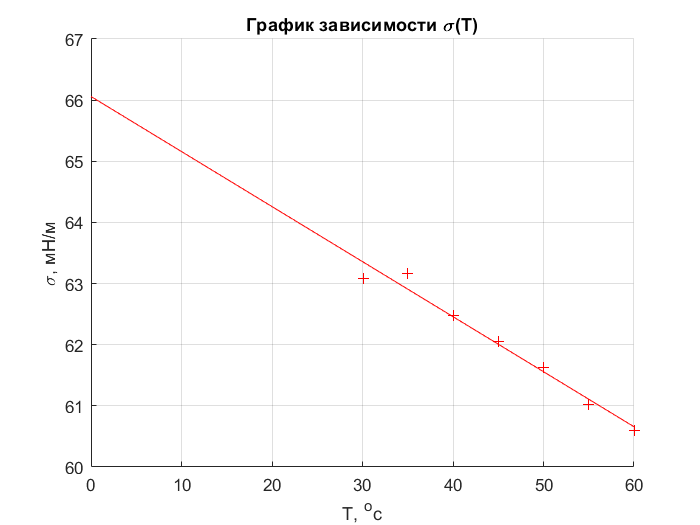
\includegraphics[scale=0.85]{../../../../../Users/Marina/plot_1.png} 
\end{center}
\end{figure}
\item Видим, что несмотря на малое число точек, у нас прослеживается линейная зависимость угловой дисперсии от порядка m
\end{enumerate}
\paragraph{Выводы:}
\begin{enumerate}
\item Мы ознакомились с устройством,работой и настройкой гониометра Г5
\item Исследовали спектр ртутной лампы.
\item Нашли период решетки, равный d = 2.200 $\pm$ 0.075 мкм 
\item Установили линейную зависимость угловой дисперсии от порядка 
\end{enumerate}
\end{document}